\documentclass[a4paper,12pt]{article}
\usepackage{lipsum}
\usepackage{listings}
\usepackage[T1]{fontenc}
\usepackage{fontspec}
\usepackage[greek]{babel}
\usepackage[super]{nth}
\usepackage{fancyhdr}
\usepackage[left=1.50cm, right=1.50cm, top=2cm, bottom=1.cm, includeheadfoot]{geometry}
\usepackage{amsmath}
\usepackage{graphicx}
\usepackage{subcaption}
\usepackage{float}
\usepackage[colorinlistoftodos]{todonotes}
\usepackage{xcolor}
\usepackage{ulem}
\usepackage{amsmath}
\usepackage{caption}
\usepackage{subcaption}
\usepackage{tabularray}
\usepackage[framed]{matlab-prettifier}
\usepackage{svg}

\usepackage[pdfauthor={Αλεξάνδρα Γιάννη, Νίκος Στυλιανού},
pdftitle={Πρώτο σετ ασκήσεων},
pdfcreator={TeX},
pdfsubject={ECE447 - ΝευροΑσαφής Υπολογιστική}]{hyperref}


\hypersetup{
	colorlinks,
	citecolor=blue,
	filecolor=black,
	linkcolor=black,
	urlcolor=blue
}

\lstset{
	style              = Matlab-editor,
	basicstyle         = \footnotesize,
	escapechar         = ",
	mlshowsectionrules = true,
}

\setmainfont{Linux Libertine O}

\pagestyle{fancy}
\fancyhf{}
\fancyhead[l]{\footnotesize 1ο σετ ασκήσεων}
\fancyhead[r]{\footnotesize Νευρο-ασαφής υπολογιστική}
%\fancyfoot[r]{\footnotesize \thepage}
\renewcommand{\footrulewidth}{0.4pt} % Line at the footer visible

\fancyfoot[c]{\thepage}

\fancypagestyle{first}{
	\fancyhf{}
	\renewcommand{\headrulewidth}{0pt}
	\fancyfoot[c]{{\large \today}}
	\renewcommand{\footrulewidth}{0.0pt} % Line at the footer visible
} 

\newcommand{\MathSpace}{\hspace{1mm}}
\setlength{\parindent}{0pt}



\begin{document}
	
	\begin{titlepage}
		\thispagestyle{first}
		
		\newcommand{\HRule}{\rule{\linewidth}{0.5mm}} % Defines a new command for the horizontal lines, change thickness here
		
		\center % Center everything on the page
		
		%----------------------------------------------------------------------------------------
		%	HEADING SECTIONS
		%----------------------------------------------------------------------------------------
		
		\textsc{\LARGE University of Thessaly}\\[1.6cm] % Name of your university/college
		
\includegraphics[scale=.5]{Images/uth-logo.png}\\[1cm] % Include a department/university logo - this will require the graphicx package
		\textsc{\Large Νευρο-ασαφής Υπολογιστική}\\[0.6cm] % Major heading such as course name
		\textsc{\large ECE447}\\[0.5cm] % Minor heading such as course title
		
		%----------------------------------------------------------------------------------------
		%	TITLE SECTION
		%----------------------------------------------------------------------------------------
		
		\HRule \\[0.5cm]
		{ \huge Σετ προβλημάτων 1}\\[0.4cm] % Title of your document
		\HRule \\[1.8cm]
		
		%----------------------------------------------------------------------------------------
		%	AUTHOR SECTION
		%----------------------------------------------------------------------------------------
		
		
		\vspace*{1cm}
		\begin{minipage}{\textwidth}
			\centering
			\begin{tblr}{cc}
				 \emph{{\LARGE Αλεξάνδρα Γιάννη}} & \emph{{\LARGE Νίκος Στυλιανού}} \\ [3mm]
				 \emph{{\LARGE AEM: 3382}} & \emph{{\LARGE AEM: 2917}} \\
			\end{tblr}
%			\begin{center} \large
%				\emph{{\LARGE Αλεξάνδρα Γιάννη }} \\[3mm]
%				\emph{\LARGE ΑΕΜ: 3382}
%			\end{center}
		\end{minipage}\\[2.5cm]
		
		% If you don't want a supervisor, uncomment the two lines below and remove the section above
		%\Large \emph{Author:}\\
		%John \textsc{Smith}\\[3cm] % Your name
		
		%----------------------------------------------------------------------------------------
		%	DATE SECTION
		%----------------------------------------------------------------------------------------
		
		
		%\vfill % Fill the rest of the page with whitespace
		
	\end{titlepage}
	
	% !TeX spellcheck = en_US
\section{Problem 1}

Contour lines of $f(x,y)$ are plotted with the following MATLAB code and are presented in figure~\ref{fig:prob_1_contour_lines}.

\begin{lstlisting}[]
function [Z] = plot_contour(start_num, end_num)
	
	x = linspace(start_num, end_num, 100);
	y = x;
	[X, Y] = meshgrid(x, y);
	Z = X.^2 + 4*X.*Y + Y.^2;
	contour(X, Y, Z, 40);
	xlabel('X');
	ylabel('Y');
end
\end{lstlisting}
\begin{figure}[h]
	\centering
	\begin{subfigure}{0.4\textwidth}
		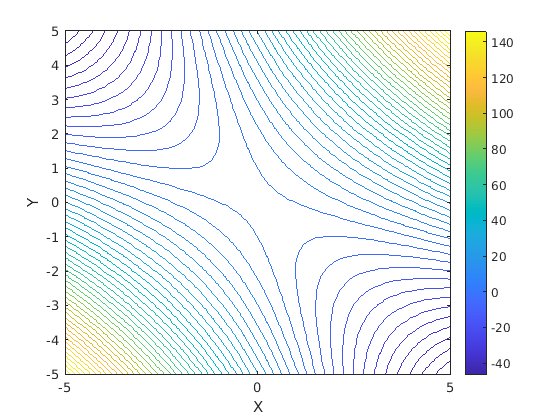
\includegraphics[width=\textwidth]{../Problem 1/contour_lines_2d.png}
		\caption{2D Plot}
		\label{fig:prob_1_contour_lines_2d}
	\end{subfigure}
	\begin{subfigure}{0.4\textwidth}
		\includesvg[width=\textwidth]{../Problem 1/contour_lines_3d.svg}
		\caption{3D Plot}
		\label{fig:prob_1_contour_lines_3d}
	\end{subfigure}
	\caption{Contour lines of $f(x,y)$ }
	\label{fig:prob_1_contour_lines}
\end{figure}

A general formula of a quadratic equation is $f(x,y) = ax^2 + 2bxy + cy^2$. Writing our formula in the previous form, we find that $a=1, \MathSpace b=2, \MathSpace c=1$.
Calculation of discriminant can help us calculate the location of function's local minimum/maximum.

\begin{equation}
\begin{gathered}
D =
\left[
\begin{array}{cc}
	f_{xx} & f_{xy} \\
	f_{yx} & f_{yy} \\
\end{array}
\right]
= f_{xx} f_{yy} - f^2_{xy} = 2 \times 2 - 4^2 = -12 < 0, \quad \text{όπου} \\
f_{xx} = \frac{\partial^2 f}{\partial x^2} = 2, \quad
f_{yy} = \frac{\partial^2 f}{\partial y^2} = 2, \quad
f_{xy} = \frac{\partial}{\partial y} \left( \frac{\partial f}{\partial x} \right) = 4
D = 2 \times 2 - 4^2 = -12 < 0.
\end{gathered}
\end{equation}

So, we only have to find the point where $\frac{\partial f}{\partial x}$ and $\frac{\partial f}{\partial y}$ are equal to $0$. Thus, this point will be a saddle point where gradients in each orthogonal direction are $0$, but this point is not either a local minimum or maximum.
Specifically:
\begin{equation}
\left\{
\begin{array}{c}
	\frac{\partial f}{\partial x} = 2x + 4y = 0 \\ 
	\frac{\partial f}{\partial y} = 4x + 2y = 0 \\
\end{array}
\right.
\Rightarrow
\left\{
\begin{array}{c}
	x = 0\\y=0\\
\end{array}
\right.
\end{equation}
Thus, the point $(x,y) = (0,0)$ is the saddle point mentioned before for the function given and this can be justified using the plotted contour lines.
	
\end{document}